\chapter{Grundlagen} \label{sec:basics}
\section{Q-Learning}
Einer der ersten Durchbrüche im Bereich des Reinforcement Learning war die Entwicklung des Q-Learning-Algorithmus \cite{06_sutton2018reinforcement}. Diesen wollen wir im Folgenden erklären.

\subsection{Das Prinzip von Q-Learning}
Dieses Kapitel stützt sich zu einem Großteil auf das Buch \textit{Reinforcement Learning: An Introduction, Second Edition} \cite{06_sutton2018reinforcement}. Falls nicht anders angegeben, wurden die Informationen hieraus entnommen.

\paragraph{Markov Decision Processes}
Alle Experimente in dieser Arbeit zielen darauf ab, Probleminstanzen von \textit{Markov Decision Processes} -- oder kurz MDPs -- zu lösen. In MDPs gibt es eine handelnde Instanz, den \textit{Agenten}, welcher mit seiner \textit{Umgebung} interagiert. Diese Interaktion erfolgt sequenziell in Zeitschritten $ t = 0, 1, 2, 3, ... $. Der Agent erhält in jedem Zeitschritt $ t $ eine Repräsentation seiner Umgebung, den Zustand $ S_t $, und führt basierend darauf eine \textit{Aktion} $ A_t $ aus. Für diese erhält er von der Umgebung einen Reward $ R_{t + 1} $, sowie einen Folgezustand $ S_{t + 1} $. Abbildung \ref{img:mdp} zeigt eine schematische Repräsentation dieses Ablaufs.
\begin{figure}[h!]
    \centering
    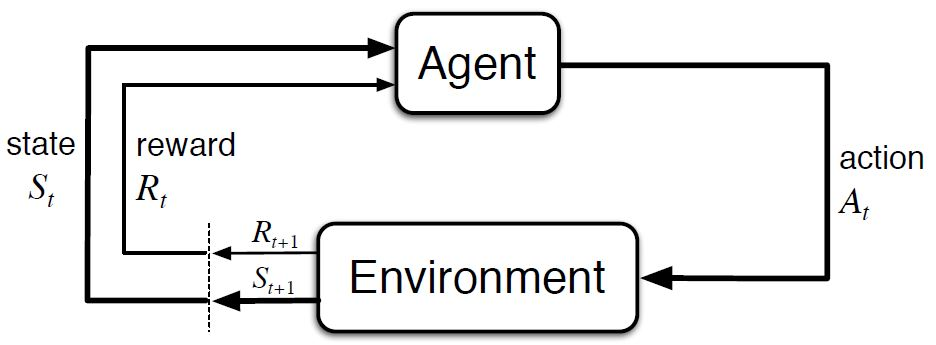
\includegraphics[width=0.5\textwidth, keepaspectratio=true]{mdp.JPG}
    \caption{Interaktion zwischen Umgebung und Agent in einem MDP} \label{img:mdp}
    \source{\cite{06_sutton2018reinforcement}}
\end{figure}

Ziel des Agenten ist es nun, seinen erwarteten Ertrag $ G_t $ zu maximieren. Im einfachsten Fall ist dies die Summe aller Belohnungen der zukünftigen Zeitschritte:
\begin{align}
    G_t \doteq R_{t + 1} + R_{t + 2} + R_{t + 3} + ... + R_T \text{,} \label{eq:expected_reward}
\end{align}
wobei T der letzte Zeitschritt einer Episode ist. In vielen Fällen ist die Interaktion zwischen Agent und Umgebung allerdings nicht endlich. Somit ist in diesen Fällen $ T = \infty $ und der Ertrag, den der Agent maximieren soll, nach Gleichung \ref{eq:expected_reward} ebenfalls potenziell unendlich. Wir führen deswegen das \textit{discounting} ein. Für $ G_t $ ergibt sich hiermit:
\begin{align}
    \begin{split}
        G_t & \doteq R_{t + 1} + \gamma R_{t + 2} + \gamma^2 R_{t + 3} + ...\\
        & = \sum_{k = 0}^{T} \gamma^k R_{t + k + 1} \text{,}
    \end{split} \label{eq:expected_discounted_reward}
\end{align}
wobei die \textit{discount rate} $ \gamma $ ein Wert zwischen $ 0 $ und $ 1 $ ist. Eine Belohnung $ k $ Zeitschritte in der Zukunft ist also nur $ \gamma^{k - 1} $--mal so viel wert wie eine Belohnung, welche im aktuellen Zeitschritt erhalten wurde.

\paragraph{Policies}
Der Agent folgt zu jedem Zeitpunkt einer Policy $ \pi $. Hierbei gibt $ \pi(a|s) $ die Wahrscheinlichkeit dafür an, dass der Agent zum Zeitschritt $ t $ die Aktion $ a \in A $ im Zustand $ s \in S $ ausführt, also dass die Aktion $ A_t = a $ wenn $ S_t = s $. Hierbei ist $ S $ die Menge aller Zustände und $ A $ die Menge aller Aktionen. $ \pi(a|s) $ ist also eine Wahrscheinlichkeitsverteilung über $ a \in A(s) $ für jedes $ s \in S $, wobei $ A(s) $ alle möglichen Aktionen im Zustand $ s $ beschreibt.

\paragraph{State-Value Functions}
Wir benötigen nun eine Möglichkeit einzuschätzen, wie gut ein Zustand $ s $ ist, wenn wir der Policy $ \pi $ folgen. Hierfür nutzen wir die \textit{state-value function} $ v_\pi $. Diese beschreibt die erwartete Belohnung eines Zustands $ s $ unter der Policy $ \pi $ zum Zeitschritt $ t $. Wir definieren $ v_\pi(s) $ als
\begin{align}
    \begin{split}
    v_\pi(s) & \doteq E_\pi \left[G_t | S_t = s \right]\\
    & = E_\pi \left[\sum_{k = 0}^{\infty} \gamma^k R_{t + k + 1} | S_t = s \right],
    \end{split}
\end{align}
wobei $ E_\pi $ der Erwartungswert vom Ertrag $ G_t $ nach Gleichung \ref{eq:expected_discounted_reward} ist, wenn der Agent sich im Zustand $ S_t = s $ befindet und der Policy $ \pi $ folgt.

\paragraph{Action-Value Functions}
Ähnlich hierzu gibt die \textit{action-value function} $ q_\pi $ an, wie profitabel es für den Agenten ist, in einem gegebenen Zustand eine gewisse Aktion auszuführen, wenn der Agent der Policy $ \pi $ folgt.

Der Wert einer Aktion $ a $ im Zustand $ s $ unter der Policy $ \pi $ ist also die erwartete Belohnung, wenn man im Zustand $ s $ zum Zeitschritt $ t $ die Aktion $ a $ ausführt und dann Policy $ \pi $ folgt. Wir definieren $ q_\pi(s, a) $ als
\begin{align}
    \begin{split}
    q_\pi(s,a) & \doteq E_\pi \left[G_t | S_t = s, A_t = a \right]\\
    & = E_\pi \left[\sum_{k = 0}^{\infty} \gamma^k R_{t + k + 1} | S_t = s, A_t = a \right].
    \end{split}
\end{align}
Die action-value function wird auch als Q-function bezeichnet, welche als Ergebnis für ein state-action Paar die Q-value liefert. Für die folgenden Implementierungen ist diese von großer Wichtigkeit.

\paragraph{Optimale Policies und Optimale Value Functions}
Das Ziel des Agenten ist, die optimale Policy $ \pi $ für ein Markov Decision Problem zu finden. Ist dieses Ziel erreicht lässt sich sagen, dass die Reinforcement Learning Aufgabe erfüllt ist. Optimal ist hierbei die Policy, welche nach Aufsummieren der Belohnungen über alle Schritte einer Episode die beste gesamte Belohnung liefert. Eine Policy $ \pi $ ist also besser als Policy $ \pi' $, wenn die erwartete Belohnung von $ \pi $ für \textbf{alle} Zustände $ s \in S $ größer ist als die von $ \pi' $. \cite{06_sutton2018reinforcement} verwendet die Formulierung
\begin{align}
    \pi \geq \pi' \text{ if and only if } v_\pi(s) \geq v_{\pi'}(s) \text{ for all } s \in S.
\end{align}

Es gibt immer eine Policy, die besser als oder gleichwertig mit allen anderen Policies ist. Diese wird -- oder im Fall, dass es mehrere gibt werden -- als $ \pi_* $ bezeichnet. Die besten Policies besitzen die gleiche state-value function, welche die \textit{optimale state-value function} $ v_* $ genannt wird und definiert wird als
\begin{align}
    v_*(s) \doteq \max_\pi v_\pi(s)
\end{align}
für alle $ s \in S $.

Optimale Policies teilen sich ebenfalls die gleiche \textit{optimale action-value function} $ q_* $, welche definiert ist als
\begin{align}
    q_*(s, a) \doteq \max_\pi q_\pi(s, a)
\end{align}
für alle $ s \in S $ und $ a \in A $. $ q_* $ liefert also für jedes state-action Paar den größtmöglichen erwarteten Ertrag, den irgendeine Policy erreichen kann.

\paragraph{Bellman Optimality Equation}
Die optimale action-value function $ q_* $ muss die folgende Gleichung erfüllen:
\begin{align}
    q_*(s, a) = E \left[R_{t + 1} + \gamma \max_{a'} q_*(s', a') \right] \label{eq:bellman}
\end{align}
Diese Gleichung wird \textit{Bellman optimality equation} für $ q_* $ genannt und besagt, dass der beste erwartete Ertrag für jedes state-action Paar $ (s, a) $ zum Zeitpunkt $ t $ der Summe aus der direkten Belohnung $ R_{t + 1} $ der Aktion $ a $ und dem \textbf{maximalen} erwarteten Ertrag, der von einem der nächsten state-action Paare $ (s', a') $ erreicht werden kann entsprechen muss. Hierbei ist $ s' $ der Folgezustand $ S_{t + 1} $ und $ a' $ die Aktion $ A_{t + 1} \in A(s') $, welche den meisten Ertrag bringt.

Das folgende Kapitel beschreibt, wie die Bellman equation verwendet wird, um $ q_* $ zu finden, was uns wiederum die optimale Policy liefern soll. 

\subsection{Der Ablauf von Q-Learning} \label{sec:q_learning_process}
Das Ziel von Q-Learning ist, die optimale Policy zu finden, indem der Agent die optimalen Q-values für jedes state-action Paar erlernt.

Der Q-Learning-Algorithmus benutzt die Bellman equation als Update-Regel, um nach und nach die Q-values für jedes state-action Paar anzunähern. Dieses Verfahren nennt man \textit{value iteration}.

Bei überschaubaren Umgebungen ist es möglich, die Werte für jedes state-action Paar in einer Tabelle, der so genannten \textit{Q-table} zu speichern. Zu Beginn weiß der Agent nichts über eine Umgebung. Die Q-table ist dementsprechend leer beziehungsweise ist der Wert jedes state-action Paares 0. Der Agent operiert nun eine vorbestimmte Anzahl von \textit{Episoden} in der Umgebung und produziert im Laufe der Zeit neue Q-values, mit denen die Q-table aktualisiert wird.

Zu Beginn jedes Schritts wählt der Agent eine Aktion für den aktuellen Zustand aus. Intuitiv macht es Sinn, die beste bisher bekannte Aktion zu wählen, um die Belohnung zu maximieren. Dieses Vorgehen ist allerdings nicht zielführend, da der Agent am Anfang nichts über seine Umgebung weiß. Er benötigt also für die Wahl seiner Aktionen eine bessere Strategie. Auf dieses Problem gehen wir in Kapitel \ref{sec:exploration_exploitation} näher ein.

Nehmen wir an, der Agent hat im Zustand $ s $ zum Zeitschritt $ t $ eine Aktion $ a $ ausgewählt. Nach der Bellman equation \ref{eq:bellman} ist dann die Q-value $ q(s, a) $ (der Übersicht in Gleichung \ref{eq:bellmanClean} und \ref{eq:updateQValue} wegen lassen wir die Policy $ \pi $ hier weg, gemeint ist natürlich $ q_\pi(s, a) $) die für die Aktion erhaltene Belohnung $ R_{t + 1} $ plus der maximale erwartete Ertrag eines folgenden state-action Paares, also
\begin{align}
    q(s, a) = R_{t + 1} + \gamma \max_{a'} q(s', a'). \label{eq:bellmanClean}
\end{align}
Dies berücksichtigt allerdings nicht, dass der Agent in einem früheren Zeitschritt oder in einer anderen Episode vielleicht bereits einen Wert $ q(s, a) $ für dieses state-action Paar berechnet und in der Q-table gespeichert hat. So wird bei jeder Berechnung eventuell ein alter Wert überschrieben und vergangene Erkenntnisse haben keinen Einfluss auf die aktuelle Berechnung.

Ein besserer Ansatz ist die Verwendung einer \textit{learning rate}. Die learning rate ist ein Wert zwischen 0 und 1, der festlegt, wie schnell der Agent vergangene Q-values aus der Q-table verwirft. Anders gesagt legt sie fest, wie viel Information aus vorherigen Berechnungen bei einem Update einer Q-value erhalten bleibt. Wir verwenden für die learning rate das Symbol $ \alpha $.

Für die Berechnung der neuen Q-value für das state-action Paar $ (s, a) $ zum Zeitpunkt $ t $ ergibt sich dann
\begin{align}
    q_\text{neu}(s, a) = (1 - \alpha) q(s, a) + \alpha \left(R_{t + 1} + \gamma \max_{a'} q(s', a') \right). \label{eq:updateQValue}
\end{align}
Bei einer learning rate von $ \alpha = 0.6 $ bleiben so $ 40\% $ des alten Wertes erhalten, während der neu erlernte Wert mit $ 60\% $ gewichtet wird.

\subsection{Exploration vs Exploitation} \label{sec:exploration_exploitation}
In Kapitel \ref{sec:q_learning_process} sind wir auf die Notwendigkeit einer Strategie, mit der der Agent seine nächste Aktion auswählt, gestoßen. Wie dort bereits erwähnt ist eine sehr simple Methode die Auswahl der Aktion mit der größten erwarteten Belohnung. Eine solche Aktion wird \textit{greedy} Aktion genannt. Gibt es mehrere greedy Aktionen mit demselben erwarteten Ertrag, so wird eine davon zum Beispiel per Zufall ausgewählt.

Diese Strategie klingt auf den ersten Blick sinnvoll, ist aber nicht so zielführend wie es scheint. Der Agent versäumt es andere Aktionen auszuprobieren, die eventuell eine bessere Belohnung liefern könnten. Er nutzt nur die ihm bekannten aus (\textit{exploitation}). Besser wäre es, wenn er ebenfalls Zeit in die Erkundung (\textit{exploration}) der Umgebung stecken würde.

Dies kann realisiert werden, indem der Agent die meiste Zeit \glqq gierig\grqq{} (\textit{greedy}) agiert und die Aktion mit dem besten geschätzten Ertrag wählt, mit einer Wahrscheinlichkeit von $ \epsilon $ allerdings ab und zu zufällig eine von allen verfügbaren Aktionen auswählt. $ \epsilon $ ist hierbei ein Wert zwischen 0 und 1, der entweder statisch oder dynamisch definiert wird. Auf diese Weise wird erreicht, dass der Agent auch Aktionen ausprobieren kann, welche er zuvor noch nicht gesehen hat. Diese Strategie wird \textit{$ \epsilon $-greedy-Strategie} genannt und zählt nach \cite{07_dabney2020temporallyextended} auch heute noch bei der Erkundung der Umgebung zu den am meisten benutzten.

\subsection{Implementierung in Python} \label{sec:qLearningImplementation}
Mit diesem Wissen werden wir nun einen Q-Learning-Algorithmus in Python implementieren.

\paragraph{Hyperparameter} \label{sec:qLearningHyperparameter}
In den vorherigen Kapiteln haben wir einige Variablen eingeführt, von denen uns manche als so genannte \textit{Hyperparameter} dienen werden \cite{08_ravichandiran2018hands}. Diese steuern das Verhalten des Agenten und sollten für den optimalen Lernerfolg angepasst werden. Wir verwenden hierfür eine Datenklasse, um alle Hyperparameter an zentraler Stelle verwalten zu können:
\begin{minted}{python}
@dataclass
class Parameters:
    num_episodes: int
    max_steps_per_episode: int

    learning_rate: float
    discount_rate: float

    start_exploration_rate: float
    max_exploration_rate: float
    min_exploration_rate: float
    exploration_decay_rate: float

    rewards_all_episodes: list
    max_rewards_all_episodes: list
\end{minted}
\mintinline{python}{num_episodes} gibt die Anzahl der Episoden an, die der Agent trainieren soll, \linebreak\mintinline{python}{max_steps_per_episode} die Schritte pro Episode. \mintinline{python}{learning_rate} und \mintinline{python}{discount_rate} sind selbsterklärend. Die folgenden vier Werte beziehen sich auf die $ \epsilon $-greedy Strategie. Wir wollen die Möglichkeit haben, unser $ \epsilon $ dynamisch anzupassen. Hierfür initialisieren wir die \mintinline{python}{start_exploration_rate} als unser Anfangs-$ \epsilon $, die \mintinline{python}{max_exploration_rate} als Absicherung und eventuelle Variable für die Zukunft (ist normalerweise identisch mit der \mintinline{python}{start_exploration_rate}), die \mintinline{python}{min_exploration_rate} als minimales $ \epsilon $ und die \mintinline{python}{exploration_decay_rate} als Größe die festlegt, wie schnell $ \epsilon $ schrumpfen soll. In den beiden Variablen \mintinline{python}{rewards_all_episodes} und \mintinline{python}{max_rewards_all_episodes} werden die Belohnungen des Trainings abgelegt.

\paragraph{Die \mintinline{python}{train()}-Methode}
Die \mintinline{python}{train()}-Methode ist das Herzstück des Algorithmus:
\begin{minted}{python}
def train(self, width: int, length: int, params: Parameters,
            environment, ...):
\end{minted}
\mintinline{python}{width} und \mintinline{python}{length} beschreiben die Breite und die Länge des Rasters. Dies wird in Kapitel \ref{img:terrainMain} deutlich werden. Mit diesen Daten wird die Größe der Q-table bestimmt. Mit den \mintinline{python}{params} übergeben wir der Funktion die Hyperparameter. Das \mintinline{python}{environment} ist die Umgebung, in der der Agent operieren soll. Die restlichen Parameter sind optional und beziehen sich auf die Visualisierung der Ergebnisse während des Trainings.

Wir verwenden für die Implementierung der Q-table \textit{NumPy}, die primäre Bibliothek für die Array-Programmierung in Python \cite{harris2020array}. Wir erzeugen ein zweidimensionales NumPy-Array, das für jeden Zustand unserer Umgebung eine Zeile und für jede Aktion eine Spalte enthält. Alle Elemente werden zunächst mit 0 initialisiert. Außerdem setzen wir unser $ \epsilon $ auf die in den Hyperparametern festgelegte \mintinline{python}{start_exploration_rate}. Wir erstellen außerdem einen Buffer, welcher die Tupel aus Zustand, Aktion, Belohnung und Folgezustand enthält. Dieser wird am Ende jeder Episode gemischt und dann abgearbeitet. Dieses Verfahren löst starke Pfadabhängigkeiten auf. In Kapitel \ref{sec:deepQPrinciple} gehen wir hierauf näher ein.
\begin{minted}{python}
    q_table = np.zeros((width * length, 4))
    exploration_rate = params.start_exploration_rate
    buffer = []
\end{minted}

Zu Beginn jeder Episode setzen wir den Zustand auf den Startzustand der Umgebung und erzeugen die beiden Variablen, die die Belohnungen der Episode speichern:
\begin{minted}{python}
    for episode in range(params.num_episodes):
        state = environment.reset_agent()
        rewards_current_episode = 0
        max_reward_current_episode = 0
\end{minted}

In jedem Zeitschritt wenden wir für die Wahl der Aktion unsere $ \epsilon $-greedy Strategie an. Hierfür erzeugen wir eine zufällige Zahl zwischen 0 und 1. Falls diese größer ist als unser aktuelles $ \epsilon $, wählt der Agent die beste bekannte Aktion, ansonsten wird aus den möglichen Aktionen zufällig eine ausgewählt. Die Umgebung liefert uns infolgedessen den Folgezustand und die erhaltene Belohnung. Anschließend speichern wir das Tupel im Buffer, aktualisieren den Zustand, speichern die Belohnungen und zeigen ggf. die Position des Agenten an:
\begin{minted}{python}
        for step in range(params.max_steps_per_episode):
            exploration_rate_threshold = random.uniform(0, 1)
            if exploration_rate_threshold > exploration_rate:
                action = np.argmax(q_table[state, :])
            else:
                action = random.choice(
                    environment.get_agent_possible_actions()
                )
            new_state, reward, _ = environment.agent_perform_action(action)
            sars = (state, action, reward, new_state)
            buffer.append(sars)

            q_table[state, action] = (1 - params.learning_rate) *\
            q_table[state, action] + params.learning_rate * (reward +\
            params.discount_rate * np.max(q_table[new_state, :]))

            state = new_state
            rewards_current_episode += reward
            if max_reward_current_episode < reward:
                max_reward_current_episode = reward
\end{minted}

Am Ende jeder Episode aktualisieren wir die entsprechenden Einträge in der Q-table mit den Daten aus dem Buffer. Hierfür wird die Formel für die Berechnung der Q-value aus Gleichung \ref{eq:updateQValue} angewendet:
\begin{minted}{python}
        random.shuffle(buffer)
        while len(buffer) > 0:
            (state, action, reward, new_state) = buffer.pop(0)
            q_table[state, action] = (1 - params.learning_rate) *\
            q_table[state, action] + params.learning_rate * (reward +\
            params.discount_rate * np.max(q_table[new_state, :]))
\end{minted}

Außerdem wird das neue $ \epsilon $ berechnet. Wir verwenden hierfür eine exponentielle Funktion, damit $ \epsilon $ am Anfang start abfällt und gegen Ende langsamer. Zuletzt werden die Belohnungen in den Params gespeichert und ggf. als Graph angezeigt.
\begin{minted}{python}
        exploration_rate = params.min_exploration_rate +\
        (params.max_exploration_rate - params.min_exploration_rate) *\
        np.exp(-params.exploration_decay_rate * episode)

        params.rewards_all_episodes.append(rewards_current_episode)
        params.max_rewards_all_episodes.append(max_reward_current_episode)

    return q_table, params
\end{minted}


\section{Deep-Q-Learning}
\subsection{Das Prinzip von Deep-Q-Learning} \label{sec:deepQPrinciple}
Bisher haben wir alle Q-values in einer Q-table gespeichert. Dieses Vorgehen ist relativ simpel, stößt aber nach \cite{11_maxim2018deeprl} bei großen Zustands- bzw. Aktionsräume schnell an seine Grenzen. Als Beispiel wird hier Q-Learning bei Atari-Spielen aufgeführt, bei denen die Pixel als Zustände benutzt werden. Es leuchtet ein, dass in so einem Fall aufgrund der großen Menge an state-action Paaren die Speicherung deren Q-values schwierig, wenn nicht sogar unmöglich ist.

Nach \cite{11_maxim2018deeprl} ist die Benutzung von Neuronalen Netzen eine der populärsten Methoden, um mit diesem Problem umzugehen. Wir kombinieren Q-Learning mit einem Neuronalen Netz und erhalten auf diese Weise ein so genanntes \textit{Deep-Q-Network} (\textit{DQN}).

Für das stabile und effiziente Trainieren eines DQNs gibt es nach \cite{11_maxim2018deeprl} einige Techniken und Tricks. Die Informationen diesbezüglich wurden -- falls nicht anders angegeben -- aus \cite{11_maxim2018deeprl} entnommen.

\paragraph{$ \epsilon $-greedy}
Die $ \epsilon $-greedy-Strategie bezieht sich auf das \glqq Exploration versus Exploitation\grqq{}-Dilemma und soll eine gleichmäßige Erkundung der Umgebung bewirken. Da wir uns hiermit bereits in Kapitel \ref{sec:exploration_exploitation} befasst haben, halten wir uns an dieser Stelle nicht weiter damit auf.

\paragraph{Replay buffer}
Die Daten, die der Agent im Laufe des Trainings sammelt, sind nicht unabhängig voneinander. Sie liegen höchst wahrscheinlich sehr nahe beieinander, da sie meist zur selben Episode gehören. Dazu kommt, dass die Verteilung der Daten durch die aktuelle Policy, beziehungsweise bei der Verwendung von $ \epsilon $-greedy teilweise zufällig bestimmt wird. Wir wollen allerdings kein zufälliges Vorgehen erlernen. Wünschenswert wäre eine Verteilung der Trainingsdaten identisch zu Stichproben unter Verwendung der optimalen Policy, die wir erlernen wollen.

Um dem entgegenzuwirken verwenden wir einen großen Speicher, welcher unsere vergangenen Beobachtungen enthält. Anstatt nun mit den letzten Beobachtungen zu trainieren, entnehmen wir zufällig Daten aus diesem Speicher. Diese Methode nennt man \textit{replay buffer}. In Kapitel \ref{sec:qLearningImplementation} verwenden wir ebenfalls einen solchen replay buffer.

\paragraph{Target network}
Ein ähnliches Problem stellt der Zusammenhang zwischen benachbarten Schritten dar. Die Bellman equasion aus Gleichung \ref{eq:bellman} besagt, dass wir den Wert von $ q_\pi(s, a) $ über $ q_\pi(s', a') $ berechnen können. Die Zustände $ s $ und $ s' $ sind allerdings nur einen Schritt voneinander entfernt. Sie sind also sehr ähnlich und vom Neuronalen Netz schwer zu unterscheiden. Das hat zur Folge, dass wir bei einem Update der Parameter des Netzes für die Annäherung von $ q_\pi(s, a) $ an das gewünschte Resultat indirekt auch den Wert für $ q_\pi(s', a') $ verändern können. Dies kann das Training sehr instabil machen.

Deshalb verwenden wir ein so genanntes \textit{target network}. Das target network ist eine Kopie des training networks -- bei uns später auch policy network genannt --, welches lediglich alle $ N $ Schritte oder Episoden synchronisiert wird. $ N $ ist hierbei ein weiterer Hyperparameter, den wir bei später als \mintinline{python}{target_update} bezeichnen. Mit dieser Kopie besitzen wir nun fixierte Werte für $ q_\pi(s', a') $, was das Training nach \cite{11_maxim2018deeprl} wesentlich stabiler machen sollte.

\paragraph{Der Trainingsablauf von DQN}
Wir betrachten nun einen klassischen Algorithmus für DQN. \cite{11_maxim2018deeprl} entnimmt dessen Schritte den bekannten Papern \textit{Playing Atari with Deep Reinforcement Learning} \cite{13_mnih2013atari} und \textit{Human-Level Control Through Deep Reinforcement Learning} \cite{12_mnih2015humanlevel}. Sinngemäß wiedergegeben ist der Ablauf nach \cite{12_mnih2015humanlevel} wie folgt:
\begin{enumerate}[nosep]
    \item Initialisieren der replay-memory-Kapazität
    \item Initialisieren des Hauptnetzes mit zufälligen Parametern
    \item Kopie des Hauptnetzes anlegen, das target network
    \item \textit{For each Episode do}
    \begin{enumerate}
        \item Startzustand initialisieren
        \item \textit{For each Zeitschritt do}
        \begin{enumerate}
            \item Auswahl einer Aktion via $ \epsilon $-greedy
            \item Ausführen der Aktion in einem Emulator
            \item Beobachten der Belohnung und des Folgezustands
            \item Speichern der Beobachtung im replay memory
            \item Zufällige Auswahl einer Reihe von Beobachtungen (batch) aus dem replay memory
            \item Vorverarbeitung der Zustände
            \item loss zwischen Q-values und Ziel-Q-values berechnen (Benutzung des target networks für den Folgezustand) % TODO loss?
            \item Aktualisieren der Gewichte im Netz, um den loss zu minimieren
            \item Alle $ N $ Episoden wird das target network mit dem Hauptnetz synchronisiert
        \end{enumerate}
    \end{enumerate}
\end{enumerate}
In unserem Fall kommt noch ein weiterer Schritt hinzu, in dem wir das aktuelle Netz kopieren und als \mintinline{python}{best_net} speichern, wenn der moving average einen neuen Höchstwert erreicht. Dieses Netz wird dann am Ende des Trainings zurückgegeben. Dies soll sicherstellen, dass zum Schluss das beste Trainingsergebnis ausgegeben wird, auch wenn der Agent im Laufe der Zeit wieder etwas verlernt hat. Wir ergänzen also:
\begin{enumerate}
    \item[4.] \textit{(Fortsetzung)} 
    \begin{enumerate}
        \item[c)] Bei neuer Höchstleistung des Trainings Synchronisation des Ausgabenetzes mit dem Hauptnetzes
    \end{enumerate}
\end{enumerate}

\subsection{Implementierung in Python} \label{sec:deepQImplementation}
Wir wollen nun einen DQN-Agenten in Python implementieren. PyTorch ist ein beliebtes Deep-Learning-Framework, welches Benutzerfreundlichkeit und Leistung vereint \cite{x01_pytorch}. Als Grundlage verwenden wir das Codebeispiel von \url{https://github.com/philtabor/Youtube-Code-Repository/blob/master/ReinforcementLearning/DeepQLearning/torch_deep_q_model.py} (Zugriff am 30.03.2021), welches für unsere Zwecke stark modifiziert wird. Das Zentrum des Geschehens ist wieder die \mintinline{python}{train()}-Methode. Der besseren Übersicht wegen sind hier einige weniger relevante Codeausschnitte heraus gekürzt (gekennzeichnet mit ...). Außerdem haben wir die Einrückung auf Methodenebene entfernt. Die Schritte sind entsprechend der Liste aus Kapitel \ref{sec:deepQPrinciple} nummeriert:
\begin{minted}[texcomments]{python}
def train(width: int, length: int, params, environment, ... ):
agent = Agent( ... ) # 1. bis 3.
scores, eps_history = [], []
max_average = -99999
for episode in range(params.num_episodes): # 4.
    score = 0
    environment.reset_agent() # a)
    observation = environment.get_state_for_deep_q(step=0, ... ) # a)
    for step in range(params.max_steps_per_episode): # b)
        action = agent.choose_action(observation) # i.
        state, reward, done = environment.agent_perform_action(
            action, ... )
        ) # ii. und iii.
        observation_ = environment.get_state_for_deep_q(step=step, ...)
        # iii.
        score += reward
        agent.store_transition(
            observation, action, reward, observation_, done
        ) # iv.

        agent.learn(episode) # v. bis ix.)

        observation = observation_
    scores.append(score)
    agent.exploration_rate = params.min_exploration_rate +\
        (params.max_exploration_rate - params.min_exploration_rate) *\
        np.exp(-params.exploration_decay_rate * episode)
    current_average = get_current_average( ... )
    if max_average < current_average or episode == plot_moving_avg_period:
        max_average = current_average
        agent.best_net.load_state_dict(agent.policy_net.state_dict())# c)
params.rewards_all_episodes = scores
params.max_reward_average = max_average
return agent.best_net, params
\end{minted}
Die Schritte 1. bis 3. passieren bei der Initialisierung des Agenten und sind relativ unspektakulär. Interessanter ist die \mintinline{python}{learn()}-Methode des Agenten, die in jedem Zeitschritt einmal aufgerufen wird und die Schritte v. bis ix. abdeckt. Wir werfen daher einen Blick auf deren Code. Auch hier haben wir aus Platzgründen die Einrückung auf der Ebene der Methode entfernt:
\begin{minted}{python}
def learn(self, episode):
if self.memory_counter < self.batch_size:
    return # return, falls noch nicht genügend Beobachtungen existieren
self.policy_net.optimizer.zero_grad()

max_mem = min(self.memory_counter, self.mem_size)
batch = np.random.choice(max_mem, self.batch_size, replace=False) # v.

batch_index = np.arange(self.batch_size, dtype=np.int32)
state_batch =\
    T.tensor(self.state_memory[batch]).to(self.policy_net.device)
new_state_batch =\
    T.tensor(self.new_state_memory[batch]).to(self.policy_net.device)
reward_batch =\
    T.tensor(self.reward_memory[batch]).to(self.policy_net.device)
terminal_batch =\
    T.tensor(self.terminal_memory[batch]).to(self.policy_net.device)
action_batch = self.action_memory[batch]
 # vii. Start
q_eval = self.policy_net.forward(state_batch)[batch_index, action_batch]
q_next = self.target_net.forward(new_state_batch)
q_next[terminal_batch] = 0.0
q_target = reward_batch + self.gamma * T.max(q_next, dim=1)[0]
loss = self.policy_net.loss(q_target, q_eval).to(self.policy_net.device)
loss.backward()
 # vii. Ende
self.policy_net.optimizer.step() # viii.

if episode % self.target_update == 0:
    self.target_net.load_state_dict(self.policy_net.state_dict()) # ix.
\end{minted}
Zuletzt betrachten wir noch die Klasse \mintinline{python}{DeepQNetwork}, welche das DQN modelliert:
\begin{minted}{python}
class DeepQNetwork(BasicNetwork):
    def __init__(self, learning_rate, input_dims, fc1_dims, fc2_dims,
                 n_actions):
        super(DeepQNetwork, self).__init__()
        self.learning_rate = learning_rate
        self.input_dims = input_dims
        self.fc1_dims = fc1_dims
        self.fc2_dims = fc2_dims
        self.n_actions = n_actions

        self.fc1 = nn.Linear(*self.input_dims, self.fc1_dims)
        self.fc2 = nn.Linear(self.fc1_dims, self.fc2_dims)
        self.out = nn.Linear(self.fc2_dims, self.n_actions)
        self.optimizer = optim.Adam(self.parameters(),
                                    lr=learning_rate)
        self.loss = nn.MSELoss()
        self.device =\
            T.device('cuda' if T.cuda.is_available() else 'cpu')
        self.to(self.device)

    def forward(self, state):
        x = T.sigmoid(self.fc1(state))
        x = T.sigmoid(self.fc2(x))
        actions = self.out(x)
        return actions
\end{minted}
Wir verwenden in unserem DQN zwei sogenannte Fully-connected hidden Layers. Das bedeutet, dass alle Neuronen einer Schicht mit allen Neuronen der nächsten Schicht verknüpft sind. PyTorch nutzt hierfür die Bezeichnung \mintinline{python}{Linear} layer. Die erste Ebene nimmt Eingaben mit den Dimensionen \mintinline{python}{input_dims} entgegen. Wir legen die Dimensionen der beiden hidden Layers für die folgenden Experimente auf \mintinline{python}{fc1_dims = 256} und \mintinline{python}{fc2_dims = 256} fest. Die Anzahl an Outputs der Ausgabeebene entspricht der Anzahl der Aktionen, die dem Agenten zur Verfügung stehen. In unserem Fall sind das \mintinline{python}{n_actions = 4}, also die vier möglichen Bewegungsrichtungen oben, rechts, unten und links.

Die ReLU-activation-function wird im Moment als die mit der besten Performance angesehen \cite{10_stevens2020deep}. Trotzdem benutzen wir für unsere activation function Sigmoid, da diese in unserem Anwendungsfall bessere Ergebnisse zu erzielen scheint. 

Die Hyperparameter werden in der Datenklasse \mintinline{python}{DeepQParameters} verwaltet. Diese enthält die gleichen Parameter wie \mintinline{python}{Parameters} aus Kapitel \ref{sec:qLearningHyperparameter}, wird aber noch um folgende ergänzt:
\begin{minted}{python}
@dataclass
class DeepQParameters:
    # ... wie in Parameters
    replay_buffer_size: int
    batch_size: int
    target_update: int
\end{minted}
Deren Funktion wurde im Kapitel \ref{sec:deepQPrinciple} bereits erläutert.